\begin{center}
\Huge
Tangenter og toppunkter
\end{center}
\section*{Hvordan vi finder ligningen for tangenten i et punkt}
\stepcounter{section}


Vi husker fra sidst ligningen for tangentlinjer.
\begin{setn}[Tangentligningen]
	Lad $f$ være en differentiabel funktion. Så er ligningen for tangenten i punktet $P(x_0,f(x_0))$ givet ved
	\begin{align*}
		y = f'(x_0)(x-x_0) + f(x_0)
	\end{align*}
\end{setn}
\begin{proof}
	Vi skal finde en linje med ligning på formen 
	\begin{align}\label{eq:1}
		y = ax+b,
	\end{align}
	der går gennem punktet $P(x_0,f(x_0))$, og som er tangent til grafen for $f$ i dette punkt.
	Vi ved derfor, at 
	\begin{align*}
		a = f'(x_0).
	\end{align*}
	Dette indsættes i \eqref{eq:1} og vi får ligningen
	\begin{align}\label{eq:2}
		y = f'(x_0)x + b.
	\end{align}
	Vi ved desuden, at linjen skal gå gennem $P$. Derfor må der gælde, at 
	\begin{align*}
		f(x_0) = f'(x_0)x_0+b,
	\end{align*}
	og altså, at
	\begin{align*}
		b = f(x_0)-f'(x_0)x_0.
	\end{align*}
	Dette indsættes på $b$'s plads i \eqref{eq:2}, og vi får
	\begin{align*}
		y &= f'(x_0)x + f(x_0) - f'(x_0)x_0\\
		&= f'(x_0)(x-x_0)+f(x_0).
	\end{align*}
\end{proof}

\begin{exa}
Vi ønsker at finde ligningen for tangenten til funktionen $x^2$ i punktet $(1,1)$. Vi finder først den afledede til $x^2$:
\begin{align*}
(x^2)' = 2x.
\end{align*}
Derfor må hældningen af tangenten i punktet $(1,1)$ være $a = f'(1) = 2$. Vi skal nu finde $b$ i ligningen $y=2x+b$, så vi indsætter vores kendte punkt:
\begin{align*}
y = 2x+b \Leftrightarrow 1= 2\cdot 1 +b \Leftrightarrow b = -1,
\end{align*}
og derfor må tangentens ligning i punktet $(1,1)$ være givet som
\begin{align*}
y = 2x-1.
\end{align*}
Funktionen $x^2$ og tangenten i punktet $(1,1)$ til $x^2$ fremgår af Fig. \ref{fig:tangent}.

\begin{figure}[H]
	\centering
	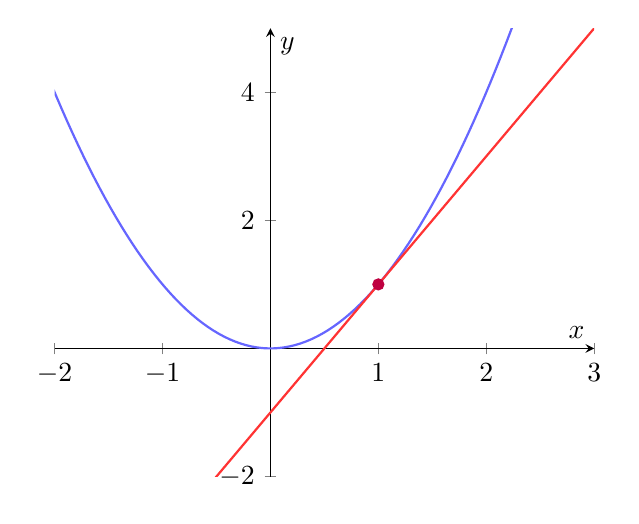
\begin{tikzpicture}
		\begin{axis}[
		axis lines = middle, 
		xmin = -2, xmax = 3, 
		ymin = -2, ymax = 5,
		xlabel = {$x$},
		ylabel = {$y$}
		]
			\addplot[color = blue!60, samples = 200,thick] {x^2};
			\addplot[color = red!80, samples = 200,thick] {2*x-1};
			\filldraw[color = purple] (axis cs:1,1) circle (2pt); 
		\end{axis}
	\end{tikzpicture}
	\caption{Funktion $f(x)=x^2$ og tangentlinjen $g(x) = 2x-1$.}
	\label{fig:tangent}
\end{figure}
\end{exa}
\section*{Ekstrema for differentiable funktioner}
\stepcounter{section}

I mange sammenhænge er det en fordel at kunne bestemme \textit{toppunkter/maksima og minima} for en funktion $f$. Hvis $f$ er en differentiabel funktion, så kan vi udnytte differentialregning til at bestemme sådanne punkter. Et punkt, der enten er et maksimum eller et minimum kaldes et \textit{ekstremumspunkt}. 

Vi har følgende sætning:
\begin{setn}[Ekstremumspunkter]
	Lad $f$ være en differentiabel funktion. Hvis et punkt $P(x_0,f(x_0))$ er et ekstremumspunkt for $f$, så gælder der, at 
	\begin{align*}
		f'(x_0) = 0.
	\end{align*}
\end{setn}
Det er dog værd at bemærke, at vi ikke nødvendigvis har den omvendte implikation; hvis $f'(x_0)=0$, så er $(x_0,f(x_0))$ ikke nødvendigvis et ekstremumspunkt. Vi kalder sådanne for \textit{vendetangenter}, og vi vil se eksempler på disse senere. 

\begin{exa}
	Lad $f$ være givet ved
	\begin{align*}
		f(x) = x^3-6x^2+5.
	\end{align*}
	Vi ønsker at bestemme ekstrema for $f$. Vi differentierer derfor først $f$.
	\begin{align*}
		f'(x) = 3x^2-12x = 3x(x-4).
	\end{align*}
	Dette sættes nu lig $0$, og vi får
	\begin{align*}
		3x(x-4) = 0, 
	\end{align*}
	og ved hjælp af nulreglen ved vi, at $x=0$ eller $x = 4$. Vi bestemmer nu de tilhørende $y$-værdier og vi får
	\begin{align*}
		f(0) = 5
	\end{align*}
	og 
	\begin{align*}
		f(4) &= 4^3 - 6\cdot 4^2+5\\
		&= 64-96+5\\
		&= -27.
	\end{align*}
	Vi har derfor en vandret tangent i $P(0,5)$ og $Q(4,-27)$. For at bestemme, om det er et ekstremumspunkt, så tegner vi grafen. Denne kan ses af Fig. \ref{fig:ekstrema}
	\begin{figure}[H]
		\centering
		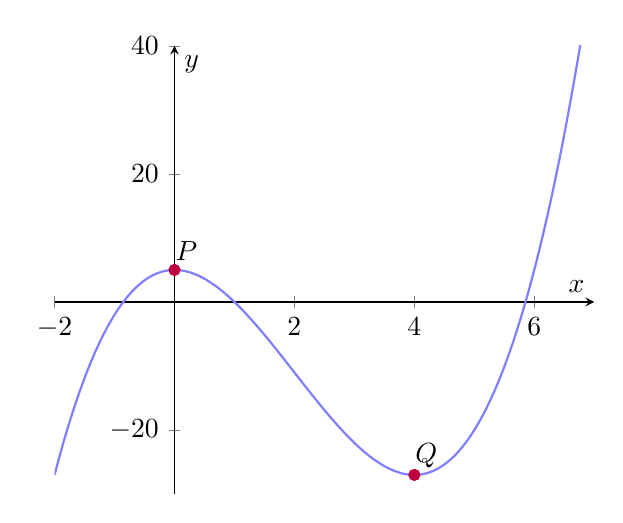
\begin{tikzpicture}
			\begin{axis}[axis lines = middle,
			xmin = -2, xmax = 7,
			ymin = -30, ymax = 40,
			xlabel = $x$, 
			ylabel = $y$]
				\addplot[color = blue!50, samples = 200, domain = -2:7, thick] {x^3-6*x^2+5};
				\filldraw[color = purple] (axis cs:0,5) circle (2pt);
				\filldraw[color = purple] (axis cs:4,-27) circle (2pt);
				\node at (axis cs: 0.2,8) {$P$};
				\node at (axis cs: 4.2,-24) {$Q$};
			\end{axis}
		\end{tikzpicture}
		\caption{Graf for funktionen $f$.}
		\label{fig:ekstrema}
	\end{figure}
\end{exa}
Af Fig. \ref{fig:ekstrema} kan vi se, at punkterne $P$ og $Q$ er ekstremumspunkter. $P$ er et \textit{lokalt maksimum} og $Q$ er et \textit{lokalt minimum}. Vi kan også se, at $f$ ikke har nogle 
\textit{globale ekstrema}.


\section*{Opgave 1}
Find ligningen for tangenten til følgende funktioner i de tilhørende punkter. Tegn desuden funktionerne og tangentlinjerne i Maple for at undersøge, om du har fundet de rigtige tangentlinjer. 
\begin{align*}
&1) \ f(x) = 7x+3,\ P(3,f(3))   &&2) \ f(x) = -3x^2+5x-1, \ P(1,f(1))     \\
&3) \ f(x) = 27, \ P(1000,f(1000))   &&4) \ f(x) = 3x^2-2\sqrt{x}, \ P(9,f(9))     \\
&5) \ f(x) = \frac{10}{x}+3x^3, \ P(2,f(2))   &&6) \ f(x) = 5x^3+2x^2+x+1, \ P(-2,f(-2))     \\
\end{align*}

\section*{Opgave 2}

Bestem ekstremumspunkter for følgende funktioner. Løs først ligningen $f'(x)=0$ og tegn derefter grafen for funktionen.  Afgør til sidst, om der er tale om globale maksimum/minimum eller lokale maksimum/minimum.

\begin{align*}
	&1) \ -x^2+10    &&2) \  x^3     \\
	&3) \  x^4-8x^2   &&4) \ \ln(x) - \frac{1}{2}x^2      \\
	&5) \ \ln(x^2)-x    &&6) \   \frac{1}{x} +x^2    \\
	&7) \  x^5-10x^4   &&8) \ \frac{1}{x^2+2x+1} - 2x      \\
\end{align*}